\documentclass[runningheads,a4paper]{llncs}
\usepackage{amssymb}
\setcounter{tocdepth}{3}
\usepackage{graphicx}
\usepackage{algorithmic}
\usepackage{algorithm}
\usepackage{graphics} % for pdf, bitmapped graphics files
\usepackage{epsfig} % for postscript graphics files
\usepackage{subfig} % for postscript graphics files
\usepackage{url}
%\urldef{\mailsa}\path|{andersonp,yongkiy,sowmya, bernhardh}@cse.unsw.edu.au|  
\newcommand{\keywords}[1]{\par\addvspace\baselineskip
\noindent\keywordname\enspace\ignorespaces#1}

\begin{document}

\mainmatter

\title{RANSAC Field-Line Detection}

%\titlerunning{RANSAC Field-Line Detection}

\author{Sean Harris \and CarlChatfield \and \\
    Bernhard Hengst}

%\authorrunning{Sean Harris et al.}

\institute{School of Computer Science and Engineering,\\
University of New South Wales, UNSW Sydney 2052 Australia}

%\toctitle{RANSAC Field-Line Detection}
%\tocauthor{Sean Harris}
\maketitle


\begin{abstract}
In the RoboCup Standard Platform League autonomous humanoid robots need to localise to play an effective game of soccer. Over the years, the league has progressively removed landmark crutches in the form of beacons, motivating the investigation of field-line features for visual sensor observations. One of the major challenges in detecting field-line features is accurately and efficiently identifying simple shapes like lines and circles. This paper describes the design and implementation of a vision field-line detection system using Random Sample Consensus (RANSAC) which is particularly effective in this challenging adversarial environment. In particular the focus will be on the use of a combined RANSAC function to detect both lines and curves in an image. These simple features are the building blocks to identify more complex field-line features including corners, T-intersections, the centre circle and the goal-box. The system is a first step towards building a complete vision-based sensor model for the aliased field-line features.  
\end{abstract}

\section{Introduction}

Over the last decade the RoboCup Standard Platform League (SPL) has progressively eliminated visual beacons that surrounded the soccer field. Autonomous robots used these beacons for localisation during soccer play. In early years there were six uniquely colour-coded beacons whereas today there are none, leaving only the goal-posts at either end of the playing area and the field-lines to help estimate the robots' position. 

Whilst the goal-posts provide observations for a robot's location on the field, they are often a long way away and can be difficult to see with low-resolution cameras, or are not in the field-of-view at all when the robot is tracking the ball. 

\begin{figure}[H]
\centering
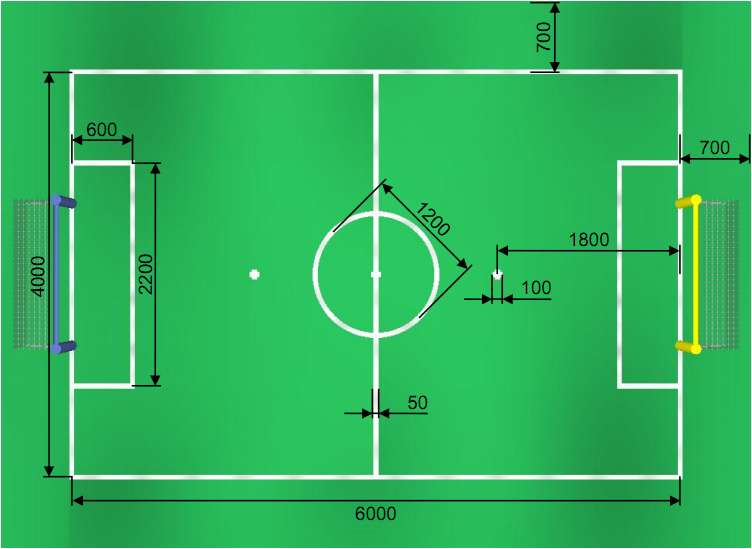
\includegraphics[width=0.45\textwidth]{Pictures/field.png}
\caption{The standard field layout for Robocup SPL 2011 showing the white field-lines.}\label{fig:field}
\end{figure}

Field lines (Figure \ref{fig:field}), on the other hand, are present all around the field in a variety of shapes and formations, often in locations that are very convenient to look at. Even though not unique, these features can provide accurate information about a robot's location. Observation of field-line features are used to provide a likelihood function of the observation given the state of the robot that is passed to a multi-modal Kalman filter \cite{claridge}\footnote{A discussion of the filter is beyond the scope of this paper}. 

One of the challenges in detecting field lines is that they are made up of two basic shapes, straight lines (side line, halfway line, goal box) and curves (centre circle). Thus, any field-line detection algorithm needs to be able to accurately distinguish between a line segment and a curve. Many efficient algorithms exist to efficiently identify straight lines \emph{or} curves in an image, however the combination of shapes present on a soccer field motivates the need to detect both shapes at once.

This paper describes the development of a combined RANSAC Lines and Circles function which is able to quickly and effectively distinguish between lines and circles in an image. The algorithm has a very high accuracy and provides a reliable set of lines and curves that can be combined to form more complex field features, including:

\begin{itemize}
   \item{Straight lines}
   \item{Corners}
   \item{T-intersections}
   \item{Parallel lines}
   \item{Centre circle}
   \item{Centre circle + halfway line}
\end{itemize}

\pagebreak
\section{Background}

We review several approaches taken by others in the detection of field-line points, simple and more complex features. 

\subsection{Generating Candidate Points} 
The first step in many feature detection algorithms used in vision is to generate a list of candidate points or regions.

Ratter, et al \cite{rUNSWift2010} use colour as the basis for generating candidate field-line points. The algorithm involves scanning vertically down an image looking for changes in colour from green to white or white to green and marking each of these points as field line points. Czarnetzki, et al \cite{NaoDevils2010} do something similar using radial scan lines instead of vertical scan lines. Both teams benefit from the speed of minimal processing, but struggle to detect vertical lines.

R{\"o}fer, et al \cite{BHumanCodeRelease2010} use a similar approach of scanning vertically through a colour classified image. They build candidate regions as opposed to identifying candidate points. Their algorithm uses the vertical scan to identify small regions and then group adjacent regions together to form larger ones. The vertical nature of their scan means that they too have to deal with the difficulty of detecting  vertical lines, especially since such lines appear as only a small number of regions.

Present methods for detecting candidate field-line points rarely work in all cases. Most approaches require the implementation of extra functionality to accurately identify points on vertical field-lines and many are also heavily reliant on colour tables.

\subsection{Detecting Simple Shapes}

Once a list of candidate points has been generated, the next step is to try and form lines and circles using these points. 

R{\"o}fer, et al \cite{BHumanCodeRelease2010} use a clustering based algorithm to group small segments that generate long field-lines. Their method includes representing each segment in Hesse normal form and grouping segments that have similar distance and direction values into longer lines. The clustering algorithm is modified to run in $O(n^2)$ time worst case and thus is not guaranteed to find optimal clusters. The left-over line segments are used to detect a circle by calculating the perpendicular bisector of each segment, intersecting it with the perpendicular bisector of each adjacent segment, and clustering them together using the original clustering algorithm. The issue is that optimal clustering techniques are sacrificed to ensure efficient run time, meaning that many sanity checks are required to ensure accurate results.

Brindza, et al \cite{UPenn2010} take a unique approach and optimise the otherwise computationally complex Hough transform \cite{HoughTransform} for use in line detection. Unfortunately they only considere one line or circle per image (possibly due to time constraints) so are not able to demonstrate its full power under competitive conditions.

There is room for several improvements in the observation of field-lines utilising efficient and accurate line and circle detection algorithms.

\subsection{Compound Field Features}
The SPL uses a standard field format for competition. The 2011 field layout is shown in Figure \ref{fig:field}. It looks similar to a normal soccer field with several identifiable field-line features including lines, corners, T-intersections, centre cirlce, penalty spot, goal box, etc. All of these features have useful information for localisation and can be vital in keeping the robot localised without having to look around for goal-posts. Few teams in the SPL can actually detect all these features.

Ratter, et al \cite{rUNSWift2010} do not detect shapes and therefore do not have the ability for field-lines to be used to localise a lost robot. They are only able to locally tune a localised robot's position using a set of points. This approach does not work if the robot is not close to where it believes it is. 

Barrett, et al \cite{uTAustin2010} are able to utilise lines and circles in each frame. The use of multiple lines instead of just a single line gives them greater precision when calculating a position from the lines. This and the centre circle also allows improved ``kidnapped" robot detection as multiple shapes can be matched to sections on the field.

Czarnetzki, et al \cite{NaoDevils2010} detect lines, corners, T-intersections, unidentified intersections and the centre circle. The corners and T-intersections are extremely useful for both fine-tuning a well localised robot's position and to solve the kidnapped robot problem. The unidentified intersection utilises every piece of information in the frame, even if the frame doesn't allow for detection of exactly which intersection is seen. They also utilise the centre circle by using its intersecting line. The combination of the line and circle generates just two symmetrical hypotheses and makes it a useful update both for a well localised robot and for a kidnapped robot.

Field-line detection is an area that the SPL can improve on. In this paper we describe the research and development of a system to fill this gap.

\section{Methodology}

We will first introduce preliminary concepts before describing our approach to field-line detection.

% Can this be referenced to carl's thesis?
%\subsection{Edge Saliency}
%Our \emph{edge saliency} image is a down-sampled $80 \times 60$ image from the original $640 \times 480$ image containing two values for each pixel. The first value represents the change across the horizontal direction ($dx$) and the second represents the change across the vertical direction ($dy$). It is generated by taking a grey scale version of the original $640 \times 480$ raw camera image, applying a Gaussian smoothing operation and calculating the $dx$ and $dy$ using a formula that models local change \cite{chatfield}. These two values allow us to determine both a magnitude and a direction for each of the pixels\footnote{the equation avoids an expensive square-root operation}:

%\begin{eqnarray}
%Magnitude^2 &=& dx^2 + dy^2\\
%Direction &=& \arctan(\frac{dy}{dx})
%\end{eqnarray}

% Can this be referenced to my thesis?
%\subsection{Image Plane vs Ground Plane}
%Points that are in the \emph{image plane} are represented in terms of their $x$ and $y$ coordinates in the saliency image. This means that a point in the very bottom right corner of the image is at $(79, 59)$ whilst a point in the very top left of the image is at $(0,0)$. In contrast to this, the \emph{ground plane} represents the 2D plane of the physical floor space around the robot. For example, in the robot-relative co-ordinate system, the point $(0,0)$ in the ground plane is directly underneath the centre of the robot, whilst the point $(1000, 0)$ is 1000 millimeters in front of the robot. Pixels in the image have a direct mapping to points on the field and this is calculated through the kinematic chain developed by \cite{rUNSWift2010}. 

\subsection{Generating Candidate Points}
The first step in the process of detecting field features is to identify candidate points that may make up part of each feature. Our algorithm utilises the common notion of scanning vertically and horizontally through the edge saliency image\cite{chatfield} and looks for pairs of matching edges corresponding to the two sides of a field line.

To start it performs a vertical scan downwards through the edge saliency image. If the edge of the field is detected, we only scan below that, if not we scan the entire image. For each pixel we consider how strong the magnitude of the edge is at that point. If it is a strong edge, we assume that the first edge found should be a green - white edge (the top of the field line). Once this first edge is found, we store its magnitude and direction for use later and move to the next point.

Upon reaching the next strong edge point, we consider whether it is part of the first edge, part of the matching white-green edge on the other side of the field line, or just a random bit of noise. We do this by examining the direction of the edge. If the edge has a \emph{similar} direction to the first edge, it is probably part of that top edge and has just spanned more than 1 pixel in width. In this case, we compare the magnitude of this point with the currently saved top edge point and only keep the largest one. However, if the next point's direction is approximately \emph{opposite} in direction to the first point, then it is considered part of the bottom side of the field-line. Similar to the top side, there can be multiple points detected as part of the bottom edge but again only the point with the highest magnitude is stored. Finally there is also a possibility that this second point fits neither of the above two categories, in which case it is assumed that the first point is noise, so we discard it and continue to search for a match to our new potential top edge.

The scan continues downwards until either it reaches the bottom image, or stops hitting strong edges. If it stops hitting strong edges then we have finished scanning the field-line. If we have detected both a top edge and a matching bottom edge we calculate the midpoint of the two to give us the centre of the field-line. To confirm the hypothesis we perform a variety of checks to ensure that we have identified a valid candidate point. They are:

\begin{itemize}
\item The top and bottom points should be opposite in direction (already tested implicitly by the algorithm)
\item	The top and bottom points should be roughly 50mm apart
%\item	The midpoint should not be too far away [what does this mean?]
\item	The midpoint should be white in the Colour Saliency
\end{itemize}

The horizontal scan runs after the vertical one and follows the same premise, but is only performed on a row if it is below the field edge and doesn't already have some field line points in it to ensure there isn't any doubling up.

\subsection{Detecting Lines and Circles}
The first step in detecting simple shapes is to convert all the points detected previously into the ground plane to assit distinguishing lines and curves. This alone however is not enough to confidently identify a line or circle segment. Figure \ref{fig:circleFail} shows the result of running the RANSAC Line\cite{RANSAC} algorithm on a frame containing primarily curves. As the image shows, there are multiple strong line candidates detected using the points that belong to the centre circle. These are incorrect line identifications since they actually belong to a circle, yet the lines fulfill all the criteria for matching, exposing a flaw in the approach.

One attempted solution was to try and run the RANSAC Circle\cite{RANSAC} algorithm first, however a circle can be detected in an image made up only of straight line segments (in particular corners or box shapes). Thus the simple RANSAC approach is not sufficient by itself to accurately distinguish lines and circles. Thus an innovative new approach has been developed whereby we run both the RANSAC Line and RANSAC Circle algorithms and compare the results to decide which shape fits the image best.

This combined RANSAC line and circle function (Algorithm \ref{alg:ransac}) is the next step in our overall process for detecting field lines.

\begin{figure}[h]
\centering
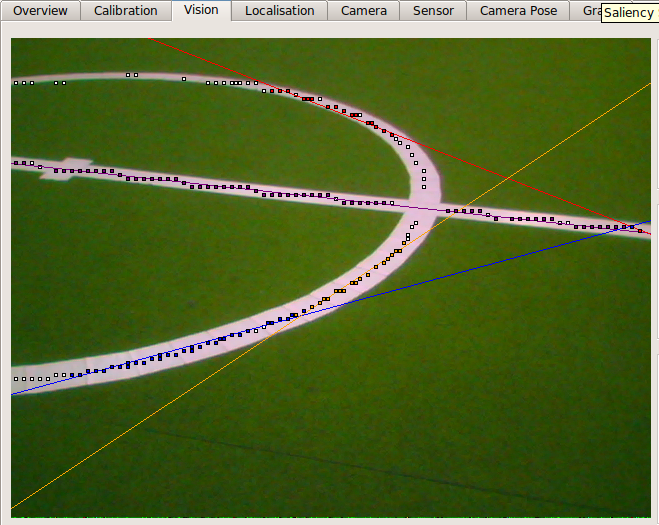
\includegraphics[width=0.5\textwidth]{Pictures/circleFail.png}
\caption{RANSAC Line detecting lines inside the centre circle when run separately to RANSAC Circle}
\label{fig:circleFail}
\end{figure}

The algorithm runs as follows: to begin we pick two points at random from the list of candidates generated above. The line defined by these two points is then calculated and the distance to each point is computed. If a point lies within the minimum distance, it is considered on the line and thus is marked and added to the variance (error function). Once all the distances have been calculated, the variance is finalised, compared with the current best and if better is saved instead. A circle of radius 600mm (see Figure \ref{fig:field}) is calculated through those points (the direction is chosen at random) and the distance from each point to the circle calculated. Similar to the line, all the points within the minimum distance are marked and added to the variance. The variance of the circle is compared against the best and saved if better. This entire process is repeated a set number of times.

\begin{algorithm} [H] 
\caption{RANSAC Line and Circle}
\begin{algorithmic} \label{alg:ransac}

\STATE $i \leftarrow 0$
\STATE $radius \leftarrow 600$
\STATE $bestLineVariance \leftarrow max$
\STATE $bestCircleVariance \leftarrow max$
\WHILE{$i < k$}
	\STATE $p1 = points[rand\%size]$
	\STATE $p2 = points[rand\%size]$
	
	\STATE $line = line(p1, p2)$
		
	\FORALL{$p \in points$}
		\STATE $distance = \frac{|line.t1*p.x + line.t2*p.y + line.t3|}{\sqrt{line.t1^2 + line.t2^2}}$
		\IF{$distance < e$}
			\STATE $variance \leftarrow variance + distance$
			\STATE $numPoints \leftarrow numPoints + 1$
		\ENDIF
	\ENDFOR
	\STATE $variance \leftarrow variance * 0.2 - numPoints$
	\IF{$variance < bestVariance$}
		\STATE $bestVariance = variance$
	\ENDIF
	
	\STATE $circle = circle(p1, p2, radius)$
	\FORALL{$p \in points$}
		\STATE $c \leftarrow circle.centre$
		\STATE $distance = \sqrt{(c.x - p.x)^2 + (c.y - p.y)^2} - radius$
		\IF{$distance < e$}
			\STATE $variance \leftarrow variance + distance^2$
			\STATE $numPoints \leftarrow numPoints + 1$
		\ENDIF
	\ENDFOR
	\STATE $variance \leftarrow variance * 0.2 - numPoints$
	\IF{$variance < bestVariance$}
		\STATE $bestVariance = variance$
	\ENDIF
	
	\STATE $i \leftarrow i + 1$
\ENDWHILE

\end{algorithmic}
\end{algorithm}


This innovative approach eliminates a problem where a RANSAC line function would pick up points better suited to the circle, whilst a RANSAC circle function would pick up points better suited to a line. The idea is to run the two algorithms in parallel, compare the final results and take the better of the two.

One of the challenges with this approach is that it requires a metric for comparing circles and lines to each other. Whilst the variance of one line is comparable to another, it isn't necessarily comparable to a circle's variance. In the end a fairly simple variance calculation involving the sum of the distances to each point and the number of points, with a slight bias towards lines, was enough to accurately compare the two shapes and ensure that even a small segment of either shape was accurately identified as the correct shape.

\subsection{Detecting Field Features}
Field-line segments are highly aliased. We would like to form highly discriminative compound features to concentrate the observation likelihood distribution. In this regard we are able to detect corners, T-intersections, pairs of parallel lines, the centre circle and halfway line, together with the simple circles and lines.

\subsubsection{Intersections - Corners and T's}
The process for finding intersections involves scanning through the list of lines detected and seeing if each one intersects any of the other lines. The critera for the point of intersection to be considered include that it has to occur not only within the image, but also at least 8 pixels from the edge and the two lines that intersect need to be approximately perpendicular.

If the checks pass, the next step is to identify the type of intersection. Since the endpoints of each line are not known it is difficult to determine if the intersection is a corner or a T. The method used to differentiate between the two relies on the fact that in a corner all the points belonging to one line should lie on one side of the other line, and vice versa. For a T intersection one line should have all its points on one side of the other, whilst the other line should have points on both sides of the first line. Thus the algorithm simply loops through the points on both lines to check which side of the opposing line they lie and uses this information to classify the intersection.

The final step is to calculate the distance, heading and orientation of the feature. If the intersection is $(X,Y)$, the formulae for these are as follows:

\begin{eqnarray}
Distance &=& \sqrt{X^2 + Y^2}\\
Heading &=& \arctan{(\frac{Y}{X})}\\
Orientation &=& \left\{ \begin{array}{rl}
heading - rotation + 180\\ \mbox{ if $rotation > 0$} \\
heading - rotation - 180\\ \mbox{ otherwise}
\end{array} \right.
\end{eqnarray}

\subsubsection{Centre Circle}
Most of the work for the centre circle detection has already been done by detecting the circle in the RANSAC section. It calculates the location of the centre of the circle in the ground plane, and its distance and heading can be calculated as above. The orientation of a circle is undefined, but if we detect the half-way field-line as well, we can give the combination an orientation. In this case we define the orientation to be the angle between the line to the centre and the half-way line. The formula is as follows:

\begin{eqnarray}
& Orientation = \nonumber \\ 
& robotToCentreDirection - centreLineDirection
\end{eqnarray}

%The method for finding the direction of the two lines used for the orientation is just a simple vector direction calculation similar to the following.

%\begin{equation}
%Direction = \arctan{(\frac{vectorY}{vectorX})}
%\end{equation}

\subsubsection{Parallel Pair}
This feature is designed to detect the goal line and the goal box line when the short vertical segment of the goal box isn't in view. Parallel pairs are determined by checking the angles of each line relative to the robot and ensuring they are roughly parallel and checking the distance between the lines is approximately 600mm. The information stored for this feature includes the specifications of the closest line as well as the perpendicular distance and heading to that line. They are calculated as follows:

\begin{eqnarray}
Perpendicular Distance = \frac{|line.t3|}{\sqrt{line.t1^2 + line.t2^2}}\\
Heading = \arctan{(\frac{-line.t1 * line.t3}{(line.t2 * line.t3})}
\end{eqnarray}


\section{Results}
Three experiments were used to test the effectiveness of the combined RANSAC Lines and Circles. In all of these experiments, the combined RANSAC was tested against the standard RANSAC Line and the standard RANSAC Circle algorithms to compare the advantages and disadvantages of the new approach.

\subsection{Curved Lines Experiment}
The first experiment involved running all three algorithms over a variety of images containing just curved lines. These images were captured using a standard Aldebaran Nao V3 from the 2011 competition camera and included the Robocup SPL field centre circle in a variety of different orientations, lengths and quantites in each image.

Figure \ref{fig:circles} shows the success rate of each of the three algorithms on the data set as a percentage. The RANSAC Circle function is obviously going to be the best for successfully identifying the curves, whilst the RANSAC Line function is obviously going to be the worst at identifying curves. The point of interest to note from this graph is that the combined function still has a fairly comparable success rate to the RANSAC Circle function, which means that there has been minimal performance degredation by adding line detecting functionality.

\begin{figure}[h!]
  \centering
  \subfloat[Only curves]{\label{fig:circles}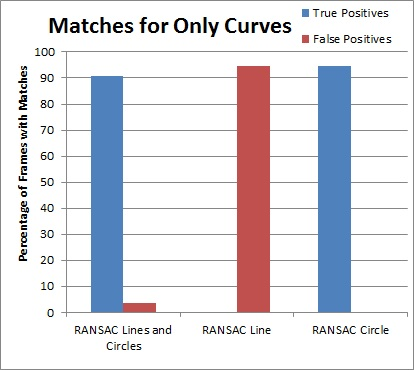
\includegraphics[width=0.4\textwidth]{Pictures/circles.jpg}}
  \subfloat[Only lines]{\label{fig:lines}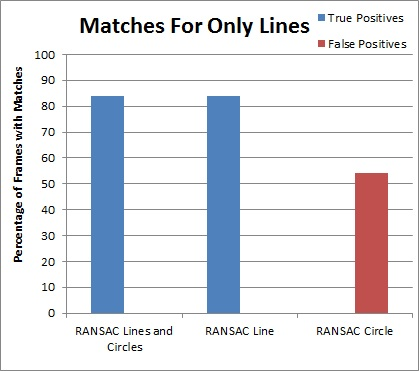
\includegraphics[width=0.4\textwidth]{Pictures/lines.jpg}}
  \caption{Percentage of matches per frame\label{both}}
\end{figure}


\subsection{Straight Lines Experiment}
The second experiment involved running all three algorithms on a variety of images containing just straight lines. Again these images were taken using the Aldebaran Nao V3 and were taken at a variety of locations around a standard SPL field. The images include straight lines, corners, T-intersections as well as combinations of the above. The goal box area is one particular area that has a lot of straight lines everywhere so has a fairly large sample size in the data set.

Figure \ref{fig:lines} shows the success rate of each of the three algorithms on this data set of only straight lines. As expected, the RANSAC Line performs the best and the RANSAC Circle performs by far the worst. As with the first experiment though, the combined RANSAC function performs only slightly worse than the RANSAC Line function but with the added functionality of being able to detect circles as well. It is also worth noting that there were no false positives from the combined RANSAC when examining only lines, meaning that the system will almost never incorrectly detect a circle. This makes any circles detected extremely reliable data to use for localisation.

\subsection{Lines and Curves Experiment}
The third experiment involved running all three algorithms on a data set of images where each frame contains exactly 1 curve and 1 straight line. Again the images were captured using the Aldebaran Nao V3 on a standard SPL soccer field and were all taken with the centre circle being the curve and the halfway line being the straight line.

This is the test where the combined RANSAC function really shows its worth. Figure \ref{fig:candl} shows that the RANSAC Line function always detected the halfway line correctly, but also always detected part of the centre circle as a straight line. This leads to its 100\% true positive and half positive score. The RANSAC Circle function always detected the centre circle correctly, but some times also detected the halway line or any left over points to be a circle as well, leading to its relatively high false positive rate. The combined RANSAC however successfully identified the centre circle and the halfway line every time without any false positives.

\begin{figure}[h]
\centering
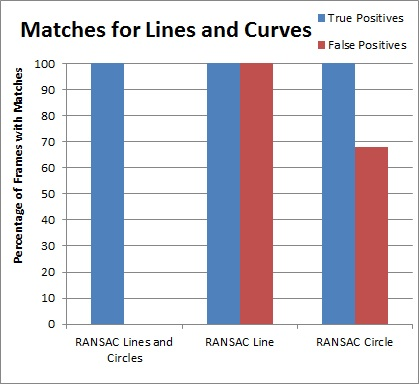
\includegraphics[width=0.5\textwidth]{Pictures/candl.jpg}
\caption{Percentage of matches per frame with both lines and curves}
\label{fig:candl}
\end{figure}

The data set size for this test was only 25 frames, which is one of the reasons for the perfect score for the combined function. The combined RANSAC function is not perfect however, so over a larger data set one would expect it would actually have a small number of false positive identifications present as well as the high true positive rate. That being said, the combined RANSAC function is clearly far more accurate and robust that either of its individual counterparts. It not only has a significantly lower false positive rate but it also has the ability to identify both shapes at once depending on the situation.

\section{Evaluation and Conclusion}
It is clear from the results presented above that neither the RANSAC Line function or the RANSAC Circle function is sufficient for detecting all the simple shapes on a standard soccer field. It would be possible to accurately detect only all the straight lines \emph{or} only all the curves, however this limits the number of landmarks available to localise the robot. It may also be possible to switch between the two functions depending on what the robot is expecting to see, but even this doesn't work if the robot sees both in one frame.

The combined RANSAC idea however provides an effective method for distinguishing between lines and curves, allowing the one algorithm to be run at all times. This not only adds simplicity to the design of the field line model, but also provides a much more robust system that is capable of dealing with all the different possible combinations of shapes on a soccer field. This algorithm proved to be the key in the development of our field line sensor model and allowed us to develop a model that can detect field features accurately and efficiently all around a soccer field.

% Add a third section combining the straight lines and curves?


%\section{Future Work}
%\subsection{Detecting the Penalty Spot}
%Penalty spot detection was not implemented primarily because they cannot be easily constructed from the line and circle models. The candidate points detected are too few for reliable classification as a line or a circle. They are discarded by the RANSAC algorithm as outliers. Penalty spot detection would be difficult to implement at a distance of more than a metre, due to the low number of candidate points it would generate. It would be quite difficult to differentiate the penalty spot from noise or even a robot section with so few points.

%At a closer distance however, the penalty spot generates a fair number of points which actually resemble a cross shape. These points could be grouped together using a simple clustering algorithm or blog detection algorithm but it might take some work to not generate false positives inside robots. There might even be enough information at close range to implement a cross based version of RANSAC to match the shape of the points to a cross.

%\subsection{Utilising Foveas}
%Another potential avenue of improvement would be to utilise the foveas developed by Chatfield \shortcite{chatfield} to detect far away balls to also detect far away field-lines. These foveas allow you to zoom in on a particular section of each image for high resolution analysis and would help remove many of the errors generated by the low resolution of the saliency image. This would allow field lines to be detected at far greater distances and could even improve the accuracy of closer field features detected.

%This would also come with its own set of challenges though, as some sort of algorithm would need to be developed to decide which area of the image is worth investigating at higher resolution. The way the vision system is currently set up, if a good algorithm for picking the area of the original image to focus on was developed, the current field-line detection code could be run using the high resolution fovea instead of the low resolution image with minimal changes.

%\subsection{Unidentified Intersections}
%One shortcoming in the current system is that we do not report an intersection between perpendicular lines unless it is clearly in the visual frame and we can identify exactly the type of the intersection it is. While this does still occur fairly often, there are also a large number of times when the point of  intersection is just outside the frame, or is close to the edge so it is hard to detect precisely what type of intersection it is. Rather than just throw this information away, it could be instead labelled as an unidentified intersection and still passed on to localisation.

%This change could be implemented easily with a few lines of code in field-line detection to instead save intersections sanity checked out because they do not land in the middle of the image. The problem with adding this is that the localisation module would require a fair bit of work to also accommodate the changes.

%\section{Conclusion}
%This paper has presented a creative and efficient methodology for detecting field-line features using RANSAC. At each stage of the process we have been able to achieve accurate and reasonably fast results which, in combintation, form a pipeline to detect a variety of field-line features across a soccer field.

\section{ACKNOWLEDGMENTS}

The authors gratefully acknowledge the support of the School of Computer Science and Engineering, other members of the 2011 rUNSWift team, and associated staff and students in the school's robotic laboratory.

%\bibliographystyle{named}


\bibliographystyle{plain}
\bibliography{references}
%\bibliography{hengst}

\end{document}
